\chapter{Evaluation}\label{sec:eval}

The most interesting projects for evaluating the implementation, are decoding softwares that are transforming a binary blob into a image. For this purpose, libjpeg, libpng and libgif are evaluated. Additionally zlib is done, since it is a general purpose library for lossless compression, which is often used in reallife products.

For those projects we are measuring two things. First, how effective our bitwidth saving is and how much we have saved. Second, we are trying to compare the assembler with and without the applied optimizations.

\section{General bitwidth}
%How much bitwidth the nodes are having in average per function
A node in $\libFIRM$ uses a amount of the available bitwidth. We note down the bitwidth of a node as $bitwidth_{irg}(n)$.
If we don't perform our analysis, then we need to assume the worst case, the node uses all the bits that are available from its mode.
If the analysis is performed, then we can say that the stable bits of the analysis are defining the bitwidth of a node.
For comparing the functions directly, we define:

$bitwidth_{irg}(irg) := \frac{\sum\nolimits_{n \in graph.nodes} bitwidth_{irn}(n)}{|graph.nodes|} $ 

We divide the sum by the number of nodes, to be able to compare smaller graphs with bigger ones. 

\paragraph{Const nodes}
\begin{figure}
	\centering
	\pgfplotstabletypeset[col sep=comma,
	columns={Library, Nodes, Ratio of Const-Nodes},
	columns/Library/.style={column type=l,string type},
%	columns/"nodes"/.style={column type=l},
%	columns/"percentNodes"/.style={column type=l},
	every head row/.style={before row=\toprule, after row=\midrule}, 
	every last row/.style={after row=\bottomrule}
	]{data.csv}
\caption{Node statistics of the project.}
\label{table:amount_const}
\end{figure}
While evaluating the projects, it came up that a normal graph consists of a lot of constant nodes, exact percentages can be found in the third column of  \autoref{table:amount_const}. 

The problem with a Constant node is, the bitwidth can be quite low. While the constant does not matter on hardware in most cases, since they are decoded directly in a hardware instruction. Additionally they don't take up any additional space in VHDL. 

Calculating how much bitwidth a constant takes is anyway only the matter of a log2(...) call, which is not really interesting to evalulate, in order to see how good the analysis works.

Summed up, Constant nodes are sophisticating the bitwidth of a function a lot. Thus the statistics later are divided into results with and without the constant values.

\paragraph{Project results}
\begin{figure}
	\centering
	\pgfplotstabletypeset[col sep=comma, fixed, zerofill, precision=4,
	columns={Library, mode usage(0), bitwidth usage(0), mode usage(1), bitwidth usage(1)},
	columns/Library/.style={column type=l,string type},
%	columns/"avgBwNc"/.style={column type=l},
%	columns/"safedBwNc"/.style={column type=l},
%	columnsLibrary.style={column type=l,string type},
%	columns/"avgBw"/.style={column type=l},
%	columns/"safedBw"/.style={column type=l},
	every head row/.style={before row={
			\toprule
			&
			\multicolumn{2}{|c|}{%
				with Const
			} &
			\multicolumn{2}{c}{%
				without Const
			}\\
		}, after row=\midrule}, 
	every last row/.style={after row=\bottomrule}
	]{data.csv}
\caption{Bitwidth saving statistics from the project}
\label{table:project_average_bitwidth}
\end{figure}
In \autoref{table:amount_const} the second column is showing the total number of nodes that got created in order to compile the library. This can be used as some sort of complexity metric. 
\autoref{table:project_average_bitwidth} shows that all the libraries except \textit{libjpeg} have a similar amount of bitwidth that got saved. However, the amount of saved bitwidth still does not really correlate with the complexity of the projects, since \textit{libgif} is not similar complex to \textit{zlib} or \textit{libpng}.\newline
We can say that we safe up about 9 bits in average per node.

\section{Optimizations on assembler output}

In this section we compare the shared object files of the library. The first run was done with plain cparser, the second run was done with cparser + the patches created for this thesis.\newline
After that the disassembly of the shared object files are compared. However, comparing those two shared object files is quite hard, due to addresses and instruction order changes. Making the comparing easier was possible after removing the address of every line and removing the arguments of the instructions. Loosing the arguments of the instruction makes it hard to compare if something in the calling of the function has changed. However, we can better study the raw changes on the instructions. What follows is the explanation, how the assembler output changes.

\paragraph{libgif} There was not a single change, the two binary files are identical.
\paragraph{libjpeg} The assembler output from after the optimization is about 30 instructions longer. The functions don't differ a lot. It looks most of the times like simple reordering of instructions. The amount of additional instructions is caused by instruction duplication, which can be caused by loop unrolling.

\paragraph{libtiff} The results here are similar to libjpeg. One difference is, the optimization causes add instructions to be translated to lea instructions. 

\paragraph{libpng} libpng seems to be different here. The assembly file after the optimization is shorter than before, by 10 instructions. Instructions that are removed are mainly mov instructions.

\paragraph{zlib} zlib is similar to libpng. The file gets 3 lines shorter, which is not much. The rest of the binary differences are basically instruction order changes.

The complete repository with the releases and data and scripts can be found at \footnote{\url{https://github.com/marcelhollerbach/bachelor-data}}.

\section{Optimization vhdl improvements}


\begin{figure}
	\centering
	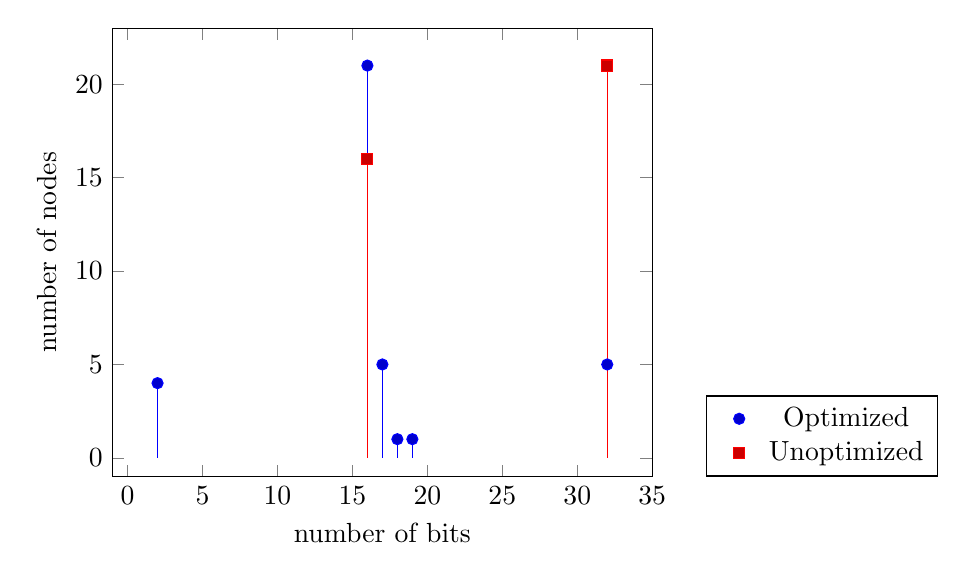
\begin{tikzpicture}
		\begin{axis}[
		legend style={at={(1.1,0)}, anchor=south west},
		xlabel=number of bits,
		ylabel=number of nodes,
		]
		\addplot+[ycomb] plot 
			coordinates {(32,5) (19,1)
				(18,1) (17,5) (16, 21) (2,4)};
		\addplot+[ycomb] plot 
			coordinates {(32,21) (16,16)};
		\legend{Optimized,Unoptimized}
	\end{axis}
	\end{tikzpicture}
	\caption{Comparison of bit usage before and after the optimization, for the code in \ref{code:vhdl-eval}}
	\label{code:vhdl-eval-table}
\end{figure}


We use a simple C snipped for evaluating the VHDL generation improvements. The C snipped can be found at \autoref{code:workflow:example}. After the C snipped was compiled into VHDL, the Xilinx Vivado 2018.2 IDE for FPGA generation was used to compile the VHDL code into a bitstream. Due to some discoveries with Vivado, a second try was done to compile the VHDL with Quartus. Quartus is a FPGA SDK from Intel Altera.

\paragraph{Vivado}
In Vivado two projects of the same kind have been created, one with the VHDL file without the improved \textit{ir2vhdl} tool, one with them. Both projects have been using the Kintex UltraScale+ xcku5p device. After the syntesis was running on both projects we took the statistic table from the report. We compared the number of LUTs and Registers. 
\begin{figure}
	\centering
	\begin{tabular}{ l c c c }
		 -        & No optimization & Optimization & Hand optimization \\
		LUTs      & 108             & 112          & 109\\
		Registers & 20              & 21           & 21\\
	\end{tabular}
	\caption{Statistics from the vivado projects}
\label{table:vhdl_improvements_vivado}
\end{figure}
In \autoref{table:vhdl_improvements_vivado} you can observe in the first two columns that the not optimized code was a lot better LUT and register wise than the optimized code. A quick look at the optimized VHDL code shows that there are a lot of redundant \textit{resize} calls. After that observation the decision was made that the redundant calls can be removed by hand right now, as from the beginning on we thought the VHDL compiler would take care of removing those. The Results of this third try can be observed in the last column.
All in all this was not improving the results at all. A deeper look showed that redundant resize calls are not handled by this VHDL compiler. Even after removing them, the amount of LUTs was still bigger than in the beginning.

\paragraph{Quartus}
As in Vivado two projects have been created. Both Project are using the Board Intel Altera Cyclone V as target device. After the Compiling and Fitting, the two Resource Usage Report have been compared.
\begin{figure}
	\centering
	\begin{tabular}{ l c c }
		-                 & No optimization & Optimization \\
		ALMs for LUT      & 54              & 54           \\
		ALMs for Registers& 4               & 4            \\
	\end{tabular}
	\caption{Statistics from the quartus projects}
	\label{table:vhdl_improvements_quartus}
\end{figure}
What can be observed in \autoref{table:vhdl_improvements_quartus} is that the optimization does not impact the numbers of ALMs used. The hand optimized code was resulting in the equal results as the optimized VHDL output, and is not explicitly listed therefore. Quartus provides a additional setting where the synthesis and fitting steps are more focused on performance or area usage. Tweaking those setting did not impact the differences between the two generated VHDL files.

Overall we can see that its quite hard to measure the improvements the VHDL optimization gives, due to the missing insight into the processes that are performed in order to compile a VHDL file into a bitstream.